% \RequirePackage{lineno}
\documentclass[onecolumn,preprintnumbers,amsmath,amssymb,superscriptaddress]{revtex4}
%\usepackage[pdftex]{graphicx}

\usepackage{amsmath,amsfonts,amssymb}
\usepackage[english]{babel}
\usepackage[latin1]{inputenc}
\usepackage[T1]{fontenc}
\usepackage{color}
\usepackage{float}
\usepackage{verbatim}
\usepackage{graphicx}
\usepackage{bm}
\usepackage{mathtools}
\usepackage{stmaryrd}
\usepackage{anyfontsize}


%\usepackage{epstopdf}
%\usepackage{array}
%\usepackage{tabularx}
%\usepackage{multirow}
\usepackage{color}
%\usepackage{multibox}
%\usepackage{rotating}
%\usepackage{lineno}
%\usepackage[left]{lineno}
\usepackage[comma,sort&compress]{natbib}
\bibpunct{}{}{,}{s}{}{;}
%\usepackage{authblk}
%\usepackage{multicol}

\bibliographystyle{naturemag}

% \usepackage{bibunits}

% \linenumbers
%  \setlength\linenumbersep{3pt}
 
\addto\captionsenglish{\renewcommand{\figurename}{Supplementary Figure\!}}

\begin{document}

% 
% \author{Justin D. Yeakel} \affiliation{School of Natural Sciences, University
%   of California, Merced, Merced, CA 95340, USA}\affiliation{The Santa Fe Institute, 1399 Hyde Park Road, Santa Fe, NM 87501, USA}\affiliation{Contributed equally}\affiliation{Corresponding author}
% 
% \author{Christopher P. Kempes} \affiliation{The Santa Fe Institute, 1399 Hyde
%   Park Road, Santa Fe, NM 87501, USA}\affiliation{Contributed equally}\affiliation{Corresponding author}
% 
% \author{Sidney Redner} \affiliation{The Santa Fe Institute, 1399 Hyde Park
%   Road, Santa Fe, NM 87501, USA}\affiliation{Contributed equally}\affiliation{Corresponding author}
% 
% \title{ Supporting Information for ``The dynamics of starvation and recovery''}%: Eco-evolutionary feedbacks}
% 
% 
% 
% \maketitle
% 

%%%%%%%%%%%%%%%%%%%%%%%%
% SUPPLEMENTARY MATERIAL
%%%%%%%%%%%%%%%%%%%%%%%%

%New additions in red text


% \clearpage

\noindent {\bf Supplementary Note 1: Sensitivity to additional death terms}

It should be noted that our set of dynamics (Eqs. 2 and 4, main text) could include a constant death term of the form $-d_{F}F$ and $-d_{H}H$ to represent death not directly linked to starvation. Adding terms of this form to our model would simply adjust the effective value of $\lambda$ and $\mu$, and we could rewrite Eq. 4 with $\lambda^{\prime}=\lambda-d$ and $\mu^{\prime}=\mu-d$. These substitutions would not alter the functional form of our model nor the steady-states and qualitative results, however the quantitative values could shift based on the size of $d$ relative to $\lambda$ and $\mu$. 

Survivorship has a well-known functional form which changes systematically with size (e.g. \citep{calder1984}). Typically survivorship is defined using the Gompertz curve 
\begin{equation}
F=F_{0}e^{\left(c_{0}/c_{1}\right)\left(1-e^{c_{1}t}\right)}
\label{gompertz}
\end{equation}
where the parameters have the following allometric dependencies on adult mass $c_{0}=a_{0}M^{b_{0}}$ and $c_{1}=a_{1}M^{b_{1}}$, with $a_{0}=1.88\times10^{-8}$ (s g$^{-b_{0}}$), $b_{0}=-0.56$, $a_{1}=1.45\times10^{-7}$ (s g$^{-b_{1}}$), and $b_{1}=-0.27$ (see \citep{calder1984} for a review).


We are interested in the specific death rate of the form $\dot{F}=-dF$, and using the derivative of Eq. \ref{gompertz} we find that $d=c_{0}e^{c_{1}t}$. Our model considers the average rates over a population and lifecycle and the average death rate is given by 
\begin{eqnarray}
\bar{d}&=&\frac{1}{t_{\text{exp}}}\int_{0}^{t_{\text{exp}}}c_{0}e^{c_{1}t} dt \\
&=&\frac{c_{0}\left(e^{c_{1} t_{\text{exp}}}-1\right)}{c_{1}t_{\text{exp}}}
\end{eqnarray}
where $t_{\text{exp}}$ is the expected lifespan following the allometry of $t_{\text{exp}}=a_{2}M^{b_{2}}$ with $a_{2}=4.04\times10^{6}$ (s g$^{-b_{2}}$) and $b_{2}=0.30$ ~\citep{damuth1982analysis,calder1984}. Given the allometries above we have that
\begin{equation}
\bar{d}=\frac{a_{0} \left(e^{a_{1}a_{2}M^{b_{1}+b_{2}}}-1\right) M^{b_{0}-b_{1}-b_{2}}}{a_{1} a_{2}}
\end{equation}
which scales roughly like $M^{b_{0}}$ because $b_{1}$ and $b_{2}$ are close in value but opposite in sign. In Supplementary Figure \ref{fig:ratescomp} we compare the value of $\bar{d}$ to the reproductive, $\lambda$, and starvation-based mortality, $\mu$, rates. The values of $\bar{d}$ are orders of magnitude smaller than these rates for all mammalian masses, and thus, adding this non-starvation based death rate to our model does not shift our results within numerical confidence.\\



\noindent {\bf Supplementary Note 2: NSM and the energy equivalence hypothesis}

The energy equivalence hypothesis is based on the observation that if one assumes that the total metabolism of an ecosystem $B_{\rm tot}$ is equally partitioned between all species ($B_{i}$, the total metabolism of one species, is a constant), then the abundances should follow $N\left(M\right)B\left(M\right)=B_{i}$ implying that $N\left(M\right)\propto M^{-\eta}$, where $\eta$ is the metabolic scaling exponent \citep{allen2002,enquist1998}. As $\eta \approx 3/4$ this hypothesis is consistent with Damuth's law \citep{allen2002}. 
However, the actual equivalence of energy usage of diverse species has not been measured at the population level for a variety of whole populations. Supplementary Figure \ref{fig:equivalence} recasts the results of the NSM in terms of this hypothesis and shows that $F^{*}B$ is nearly constant over the same range of mammalian sizes up to the asymptotic behavior for the largest terrestrial mammals.\\


\noindent {\bf Supplementary Note 3: Application of NSM limits to aquatic mammals}
A theoretical upper bound on mammalian body size is given by $\epsilon_\sigma=0$, where mammals are entirely composed of metabolic reserves, and this occurs at $M=8.3\times 10^8$ (g), or $120$ times the mass of a male African elephant. We note this particular limit as it may have future relevance to considerations of the ultimate constraints on aquatic mammals.\\

\clearpage

\noindent {\bf Supplementary Figures}\\


\begin{figure}[h!]
\centering
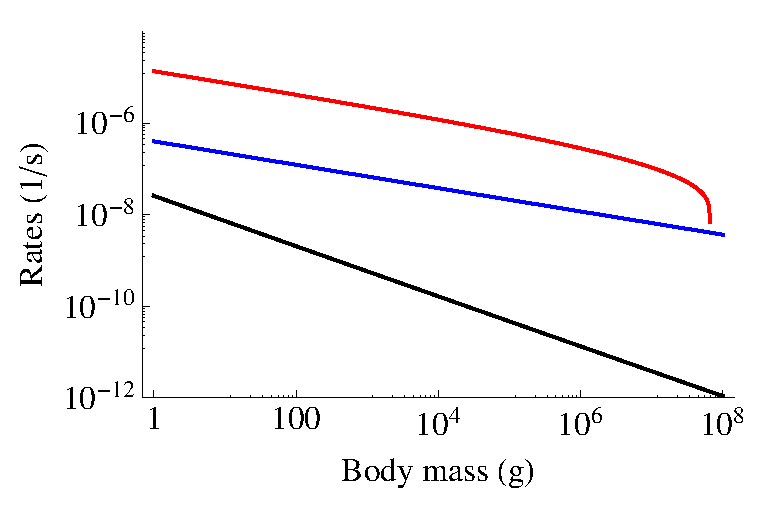
\includegraphics[width=0.4\textwidth]{mortality-rate-comparison.eps}
\caption{\small{The rates of reproduction $\lambda$ (blue), starvation-based mortality $\mu$ (red), and survivorship-based death $\bar{d}$ (black) as a function of adult mass.}\label{fig:ratescomp}}
\end{figure}

\begin{figure}[h!]
\centering
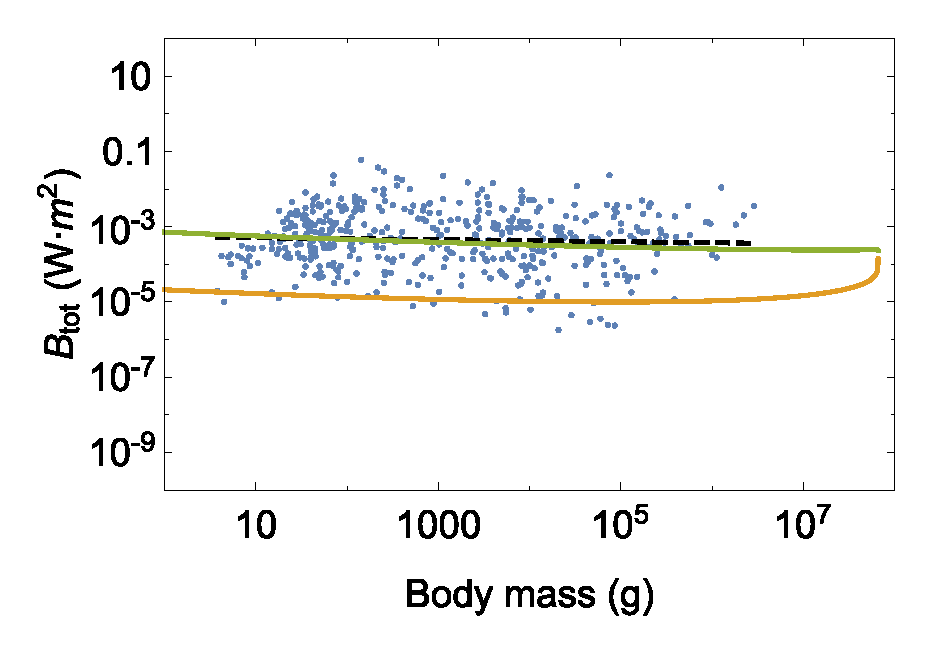
\includegraphics[width=0.4\textwidth]{fig_FPenergyequiv.eps}
\caption{\small{ Total energetic use $B_{\rm tot}$ of consumer populations at the steady state as a function of body mass ($F^*$ is shown in green and $H^*$ in orange).  The data are from Damuth \citep{Damuth:1987kr} and have been converted to
  total population metabolism using the allometric relationships for
  metabolic rate (e.g. Refs.~\citep{West:2001bv,hou,moses2008rmo}).}\label{fig:equivalence}}
\end{figure}

\clearpage

\noindent {\bf Supplementary References}\\
\def\bibfont{\footnotesize}


% \bibliography{aa_starving_supplement}
\begin{thebibliography}{10}
\expandafter\ifx\csname url\endcsname\relax
  \def\url#1{\texttt{#1}}\fi
\expandafter\ifx\csname urlprefix\endcsname\relax\def\urlprefix{URL }\fi
\providecommand{\bibinfo}[2]{#2}
\providecommand{\eprint}[2][]{\url{#2}}

\bibitem{Kempes:2012hy}
\bibinfo{author}{Kempes, C.~P.}, \bibinfo{author}{Dutkiewicz, S.} \&
  \bibinfo{author}{Follows, M.~J.}
\newblock \bibinfo{title}{{Growth, metabolic partitioning, and the size of
  microorganisms.}}
\newblock \emph{\bibinfo{journal}{PNAS}} \textbf{\bibinfo{volume}{109}},
  \bibinfo{pages}{495--500} (\bibinfo{year}{2012}).

\bibitem{kempes2014morphological}
\bibinfo{author}{Kempes, C.~P.}, \bibinfo{author}{Okegbe, C.},
  \bibinfo{author}{Mears-Clarke, Z.}, \bibinfo{author}{Follows, M.~J.} \&
  \bibinfo{author}{Dietrich, L.~E.}
\newblock \bibinfo{title}{Morphological optimization for access to dual
  oxidants in biofilms}.
\newblock \emph{\bibinfo{journal}{Proceedings of the National Academy of
  Sciences}} \textbf{\bibinfo{volume}{111}}, \bibinfo{pages}{208--213}
  (\bibinfo{year}{2014}).

\bibitem{West:2001bv}
\bibinfo{author}{West, G.~B.}, \bibinfo{author}{Brown, J.~H.} \&
  \bibinfo{author}{Enquist, B.~J.}
\newblock \bibinfo{title}{{A general model for ontogenetic growth}}.
\newblock \emph{\bibinfo{journal}{Nature}} \textbf{\bibinfo{volume}{413}},
  \bibinfo{pages}{628--631} (\bibinfo{year}{2001}).

\bibitem{moses2008rmo}
\bibinfo{author}{Moses, M.~E.} \emph{et~al.}
\newblock \bibinfo{title}{{Revisiting a model of ontogenetic growth: Estimating
  model parameters from theory and data}}.
\newblock
  \emph{\bibinfo{journal}{American Naturalist}}
  \textbf{\bibinfo{volume}{171}}, \bibinfo{pages}{632--645}
  (\bibinfo{year}{2008}).

\bibitem{hou}
\bibinfo{author}{Hou, C.} \emph{et~al.}
\newblock \bibinfo{title}{{Energy uptake and allocation during ontogeny}}.
\newblock \emph{\bibinfo{journal}{Science}} \textbf{\bibinfo{volume}{322}},
  \bibinfo{pages}{736--739} (\bibinfo{year}{2008}).

\bibitem{pirt}
\bibinfo{author}{Pirt, S.}
\newblock \bibinfo{title}{The maintenance energy of bacteria in growing
  cultures}.
\newblock \emph{\bibinfo{journal}{Proceedings of the Royal Society of London B:
  Biological Sciences}} \textbf{\bibinfo{volume}{163}},
  \bibinfo{pages}{224--231} (\bibinfo{year}{1965}).

\bibitem{Heijnen}
\bibinfo{author}{Heijnen, J.} \& \bibinfo{author}{Roels, J.}
\newblock \bibinfo{title}{A macroscopic model describing yield and maintenance
  relationships in aerobic fermentation processes}.
\newblock \emph{\bibinfo{journal}{Biotechnology and Bioengineering}}
  \textbf{\bibinfo{volume}{23}}, \bibinfo{pages}{739--763}
  (\bibinfo{year}{1981}).

\bibitem{peters1986ecological}
\bibinfo{author}{Peters, R.~H.}
\newblock \emph{\bibinfo{title}{The Ecological Implications of Body Size}},
  vol.~\bibinfo{volume}{2} (\bibinfo{publisher}{Cambridge University Press},
  \bibinfo{address}{Cambridge}, \bibinfo{year}{1986}).

\bibitem{blueweiss1978relationships}
\bibinfo{author}{Blueweiss, L.} \emph{et~al.}
\newblock \bibinfo{title}{Relationships between body size and some life history
  parameters}.
\newblock \emph{\bibinfo{journal}{Oecologia}} \textbf{\bibinfo{volume}{37}},
  \bibinfo{pages}{257--272} (\bibinfo{year}{1978}).

\bibitem{stryer}
\bibinfo{author}{Stryer, L.}
\newblock \emph{\bibinfo{title}{{Biochemistry, Fourth Edition}}}
  (\bibinfo{publisher}{W.H. Freeman and Company}, \bibinfo{address}{New York},
  \bibinfo{year}{1995}).

\bibitem{Dunbrack:1993ec}
\bibinfo{author}{Dunbrack, R.~L.} \& \bibinfo{author}{Ramsay, M.~A.}
\newblock \bibinfo{title}{{The allometry of mammalian adaptations to seasonal
  environments: A critique of the fasting endurance hypothesis}}.
\newblock \emph{\bibinfo{journal}{Oikos}} \textbf{\bibinfo{volume}{66}},
  \bibinfo{pages}{336--342} (\bibinfo{year}{1993}).

\bibitem{Lindstedt:1985hm}
\bibinfo{author}{Lindstedt, S.~L.} \& \bibinfo{author}{Boyce, M.~S.}
\newblock \bibinfo{title}{{Seasonality, fasting endurance, and body size in
  mammals}}.
\newblock \emph{\bibinfo{journal}{Am. Nat.}} \textbf{\bibinfo{volume}{125}},
  \bibinfo{pages}{873--878} (\bibinfo{year}{1985}).

\bibitem{Lindstedt:2002td}
\bibinfo{author}{Lindstedt, S.~L.} \& \bibinfo{author}{Schaeffer, P.~J.}
\newblock \bibinfo{title}{{Use of allometry in predicting anatomical and
  physiological parameters of mammals.}}
\newblock \emph{\bibinfo{journal}{Lab. Anim.}} \textbf{\bibinfo{volume}{36}},
  \bibinfo{pages}{1--19} (\bibinfo{year}{2002}).

\bibitem{estermann}
\bibinfo{author}{Estermann, B.~L.}, \bibinfo{author}{Wettstein, H.-R.},
  \bibinfo{author}{Sutter, F.} \& \bibinfo{author}{Kreuzer, M.}
\newblock \bibinfo{title}{Nutrient and energy conversion of grass-fed dairy and
  suckler beef cattle kept indoors and on high altitude pasture}.
\newblock \emph{\bibinfo{journal}{Animal Research}}
  \textbf{\bibinfo{volume}{50}}, \bibinfo{pages}{477--493}
  (\bibinfo{year}{2001}).

\bibitem{michaletz2014convergence}
\bibinfo{author}{Michaletz, S.~T.}, \bibinfo{author}{Cheng, D.},
  \bibinfo{author}{Kerkhoff, A.~J.} \& \bibinfo{author}{Enquist, B.~J.}
\newblock \bibinfo{title}{Convergence of terrestrial plant production across
  global climate gradients}.
\newblock \emph{\bibinfo{journal}{Nature}} \textbf{\bibinfo{volume}{512}},
  \bibinfo{pages}{39--43} (\bibinfo{year}{2014}).

\bibitem{damuth1987interspecific}
\bibinfo{author}{Damuth, J.}
\newblock \bibinfo{title}{Interspecific allometry of population density in
  mammals and other animals: the independence of body mass and population
  energy-use}.
\newblock \emph{\bibinfo{journal}{Biological Journal of the Linnean Society}}
  \textbf{\bibinfo{volume}{31}}, \bibinfo{pages}{193--246}
  (\bibinfo{year}{1987}).

\bibitem{calder1984}
\bibinfo{author}{Calder, W.~A.}
\newblock \emph{\bibinfo{title}{Size, function, and life history}}
  (\bibinfo{publisher}{Harvard University Press}, \bibinfo{year}{1984}).

\bibitem{damuth1982analysis}
\bibinfo{author}{Damuth, J.}
\newblock \bibinfo{title}{Analysis of the preservation of community structure
  in assemblages of fossil mammals}.
\newblock \emph{\bibinfo{journal}{Paleobiology}} \textbf{\bibinfo{volume}{8}},
  \bibinfo{pages}{434--446} (\bibinfo{year}{1982}).

\bibitem{allen2002}
\bibinfo{author}{Allen, A.~P.}, \bibinfo{author}{Brown, J.~H.} \&
  \bibinfo{author}{Gillooly, J.~F.}
\newblock \bibinfo{title}{{Global biodiversity, biochemical kinetics, and the
  energetic-equivalence rule}}.
\newblock \emph{\bibinfo{journal}{Science}} \textbf{\bibinfo{volume}{297}},
  \bibinfo{pages}{1545--1548} (\bibinfo{year}{2002}).

\bibitem{enquist1998}
\bibinfo{author}{Enquist, B.~J.}, \bibinfo{author}{Brown, J.~H.} \&
  \bibinfo{author}{West, G.~B.}
\newblock \bibinfo{title}{{Allometric scaling of plant energetics and
  population density}}.
\newblock \emph{\bibinfo{journal}{Nature}} \textbf{\bibinfo{volume}{395}},
  \bibinfo{pages}{163--165} (\bibinfo{year}{1998}).

\bibitem{Damuth:1987kr}
\bibinfo{author}{Damuth, J.}
\newblock \bibinfo{title}{{Interspecific allometry of population density in
  mammals and other animals: the independence of body mass and population
  energy-use}}.
\newblock \emph{\bibinfo{journal}{Biol. J. Linn. Soc.}}
  \textbf{\bibinfo{volume}{31}}, \bibinfo{pages}{193--246}
  (\bibinfo{year}{1987}).

\end{thebibliography}



% \end{bibunit}



\end{document}
